\chapter{CẤU TRÚC TỔNG QUAN}
    \section{Chức năng tổng quan}
        \begin{itemize}
            \item Tạo mô hệ thống WebServer giám sát và điều khiển thiết bị IOT từ xa. Cho phép người dùng đăng nhập vào hệ thống và thực hiện các thao tác điều khiển thiết bị IOT.
            \item Lưu trữ dữ liệu từ thiết bị IOT lên WebServer. Tạo giao diện tương tác với người dùng.
            \item Đóng gói WebServer thành một ứng dụng có thể chạy trên nhiều nền tảng khác nhau.
        \end{itemize}
    \section{Sơ đồ khối}
        \begin{figure}[H]
            \centering
            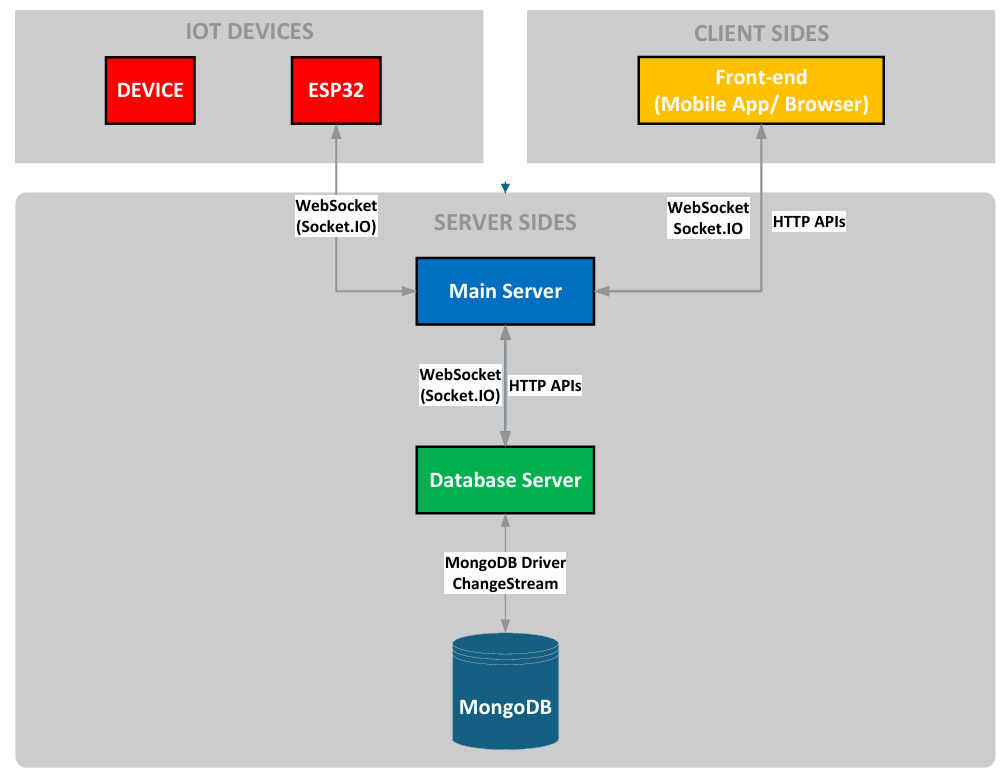
\includegraphics[width=1\textwidth]{pictures/OverviewDiagram.png}
            \caption{Sơ đồ khối WebServer}
            \label{fig:overview_diagram} 
        \end{figure}
        \begin{itemize}
            \item \textbf{ESP32}: thiết bị trung gian, nhận dữ liệu từ thiết bị IOT và gửi dữ liệu lên WebServer.
            \item \textbf{Front-end}: gửi POST/GET request đến WebServer để hiển thị giao diện tương tác với người dùng. 
            \item \textbf{MainServer}: là máy chủ chính của hệ thống, nhận dữ liệu từ ESP32, xác thực dữ liệu và chuyển tiếp dữ liệu đến DatabaServer. Nhận các yêu cầu từ Front-end và trả về dữ liệu cho Front-end.
            \item \textbf{DatabaseServer}: là máy chủ cơ sở dữ liệu, lưu trữ dữ liệu của hệ thống thông qua Database. Nhận yêu cầu từ MainServer và trả về dữ liệu cho MainServer.
            \item \textbf{Database}: là nơi lưu trữ dữ liệu của hệ thống, cho phép truy vấn và lưu dữ liệu từ DatabaseServer.
         \end{itemize}
